\chapter{SYSTEM ANALYSIS AND DESIGN}
\section{System Analysis}
We are following a structured approach that employs Rapid Application Development (RAD) methodology. This method breaks down the larger project into smaller, manageable steps, allowing for incremental progress through a series of iterations. We develop individual modules and integrate them, focusing on delivering and refining smaller portions of work. This approach ensures continuous improvement and alignment with our overall goals while effectively managing the project and incorporating ongoing feedback and adjustments.
\subsection{Requirement Analysis}
Requirement analysis is a critical phase in the software development lifecycle that focuses on understanding and documenting the needs and expectations of stakeholders. This process involves gathering detailed information about what users require from a system, which includes identifying functional requirements (what the system should do), non-functional requirements (how the system should perform), and constraints (limitations or restrictions). The goal is to create a comprehensive and clear specification that guides the development team in designing and implementing the system. Effective requirement analysis ensures that the final product aligns with user needs and business objectives, reduces the risk of project failure, and facilitates efficient communication among stakeholders. By thoroughly analyzing requirements, teams can address potential issues early, prioritize features, and ensure a smoother development process.
\subsubsection{Functional Requirements}The functional requirements of LabXplorer are mentioned below:
\begin{itemize}
    \item \textbf{User Profiles and Progress Tracking:} LabXplorer enables children and teachers to create personalized profiles for tracking their learning progress and achievements. Users can log in with unique credentials, update their profiles with educational interests and avatars, and monitor their completion of simulations and quizzes. The progress tracking feature records tasks completed, concepts learned, and achievements unlocked, offering a comprehensive view of individual learning journeys and performance over time.

    \item \textbf{Interactive Virtual Simulations:} LabXplorer offers a range of interactive virtual simulations, including Basic Electronics, Basic Chemistry, Basic Astronomy, and an Online Coding Environment. These simulations provide immersive experiences where users can engage in hands-on activities, such as manipulating virtual equipment and conducting experiments. By integrating interactive animations and real-world scenarios, LabXplorer facilitates experiential learning, allowing users to explore scientific principles and phenomena in a dynamic digital environment.

    \item \textbf{Teacher Tools and Student Assignments:} Teachers are equipped with specialized tools to create and manage educational workflows and assign tasks to students. They can design experiment workflows with sequential steps, interactive quizzes, and checkpoints to assess student progress. Teachers review completed assignments, provide feedback, and evaluate learning outcomes, ensuring that learning experiences are tailored to individual needs. Learning capsules, similar to workflows or blog entries, provide focused content and insights on specific topics, allowing for an organized and structured approach to content delivery and knowledge reinforcement.

    \item \textbf{Discussion Forum for Learning Community:} LabXplorer includes a discussion forum that promotes collaborative learning and knowledge sharing. Both students and teachers can start discussions, ask questions, share insights, and respond to others' posts. The forum supports threaded discussions, tagging, and search functionalities, fostering meaningful interactions and peer engagement within the learning community.

    \item \textbf{Quizzes and Learning Capsules:} LabXplorer integrates quizzes and learning capsules to reinforce knowledge and assess comprehension. Quizzes are designed to evaluate understanding of concepts covered in simulations, while learning capsules provide bite-sized, focused content on specific topics. These features help consolidate learning and provide instant feedback.

    \item \textbf{Admin Dashboard:} The admin dashboard in LabXplorer offers a centralized interface for managing user accounts, monitoring platform usage, and overseeing system performance. Administrators can access detailed analytics, configure system settings, and manage content to ensure smooth operation and address any issues that arise.
\end{itemize}

\subsubsection{Nonfunctional Requirements}
The nonfunctional requirements of LabXplorer are mentioned below:
\begin{itemize}
    \item \textbf{Performance Enhancement:} The focus on performance involves optimizing the platform to handle high user loads and complex simulations efficiently. This includes minimizing reliance on external frameworks and ensuring smooth and responsive interactions.
    \item \textbf{Authentication Security:} Security is a paramount concern. To enhance the platform’s security, advanced authentication algorithms, particularly focusing on hashing techniques within the backend environment, have been implemented. This ensures that user authentication data is stored and managed in a highly secure manner.
    \item \textbf{Better UX Design:} User experience is central to the project’s success. The emphasis on better UX design means that every aspect of the platform’s interface, from navigation to interaction, will be meticulously crafted to ensure a seamless and intuitive experience. This design approach caters not only to experienced users but also to newcomers, ensuring that all users can effortlessly navigate and engage with the platform.
    \item \textbf{Responsive Design:} Recognizing the diverse range of devices and browsers that users utilize, the creation of a responsive design is important for this project. This means that the platform’s design and functionality will adapt flawlessly to various screen sizes, ensuring that users can access and interact with the platform effectively, whether they are using a desktop computer, tablet, or smartphone. This responsiveness guarantees a consistent and satisfying experience aweb different devices and platforms, promoting accessibility and usability.
\end{itemize}
\section{Feasibility Analysis}
A feasibility study is a systematic and structured analysis conducted to determine the viability and practicality of a proposed project plan. It serves as an evaluation tool to assess whether the project can be successfully implemented and if it aligns with the organization's goals and objectives. It involves gathering and analyzing relevant information to determine if the project is technically feasible, operationally feasible, economically feasible, and scheduling feasible.
\subsection{Economical Feasibility}
Since the proposed system involves developing a web application, we will utilize a range of free and open-source software development tools. For the frontend, we will use \textbf{React}, a popular JavaScript library for building dynamic and interactive user interfaces. On the backend, \textbf{Express}, a minimal and flexible Node.js web application framework, will be employed to handle server-side logic and HTTP requests. For database management, we will utilize \textbf{PostgreSQL}, an open-source relational database management system known for its reliability and performance. To create interactive simulations, we will use \textbf{Phaser}, a robust HTML5 game framework, and \textbf{Unity}, a powerful cross-platform game engine, for more complex simulations and 3D elements. Additionally, we will need to allocate funds for economical server hosting to ensure the application is accessible to users while managing costs effectively.
\subsection{Operational Feasibility}
LabXplorer prioritizes operational feasibility by adopting a user-centric design approach, emphasizing simplicity and ease of use. The system is designed to be highly interactive, enabling both students and educators to navigate effortlessly without needing extensive technical knowledge. The user interface (UI) features a clean layout and intuitive controls, providing a seamless experience when accessing virtual environment and educational resources. By minimizing the need for extensive training and reducing potential barriers to adoption, LabXplorer enhances user acceptance and engagement. Overall, its straightforward design promotes effective use of the app's features, supporting educational activities and fostering a positive user experience.
\subsection{Technical Feasibility}
Combining Express.js with React and PostgreSQL offers a robust and scalable solution for developing modern applications. Express.js, built on Node.js, provides an efficient backend framework for creating RESTful APIs and managing server-side logic. PostgreSQL, renowned for its reliability and advanced data management features, serves as a solid foundation for secure and efficient data storage and querying. On the frontend, React enables the creation of responsive and visually appealing applications across multiple platforms using a single codebase. This stack leverages the strengths of each technology: Express.js for backend scalability and API development, PostgreSQL for comprehensive data handling, and React for seamless and dynamic UI development. Supported by active communities and extensive documentation, this combination ensures ample technical support, resources, and flexibility for both deployment and maintenance, making it an ideal choice for delivering modern, interactive applications.
\section{Structured System Modelling }
Structured system modeling is a methodical approach for designing complex systems by breaking them into manageable components and using formal diagrams and tools. It helps in clearly defining system requirements, workflows, and interactions.
\subsection{Processing Modling: DFD}
DFD or Data Flow Diagram is mainly used to show how data are being flowed in and out of our system. There are 3 levels of DFD i.e Context Level(Level 0),Level 1 and Level 2
\begin{figure}[H]
    \centering
    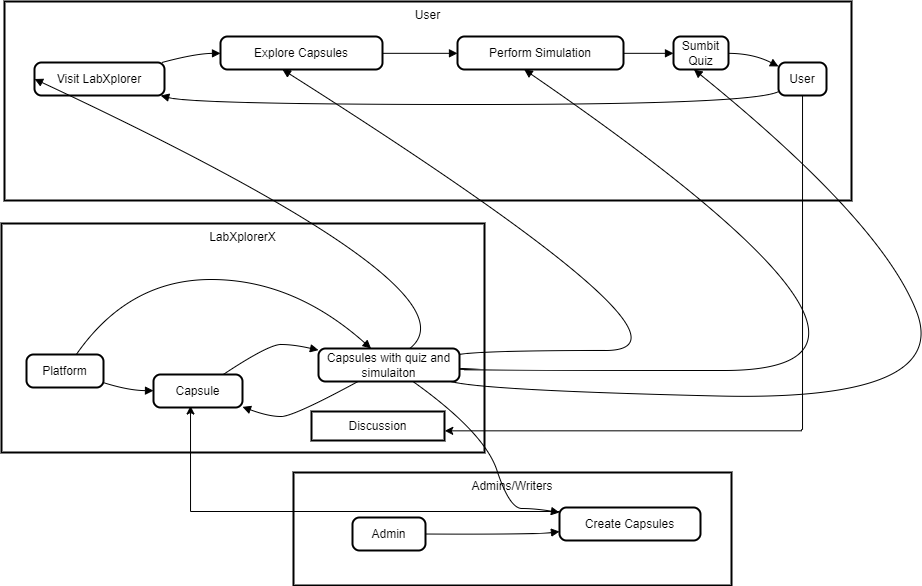
\includegraphics[height = 9cm]{Diagrams/DFD.drawio.png}
    \caption{Data Flow Diagram (Context Level)}
\end{figure}
\newpage
\subsection{Data Modelling(ER-Diagram)}
ER Diagram is mainly used to design database schema. With the help of below er diagram we can easily design database in SQL.
\begin{figure}[H]
    \rotatebox{90}{
    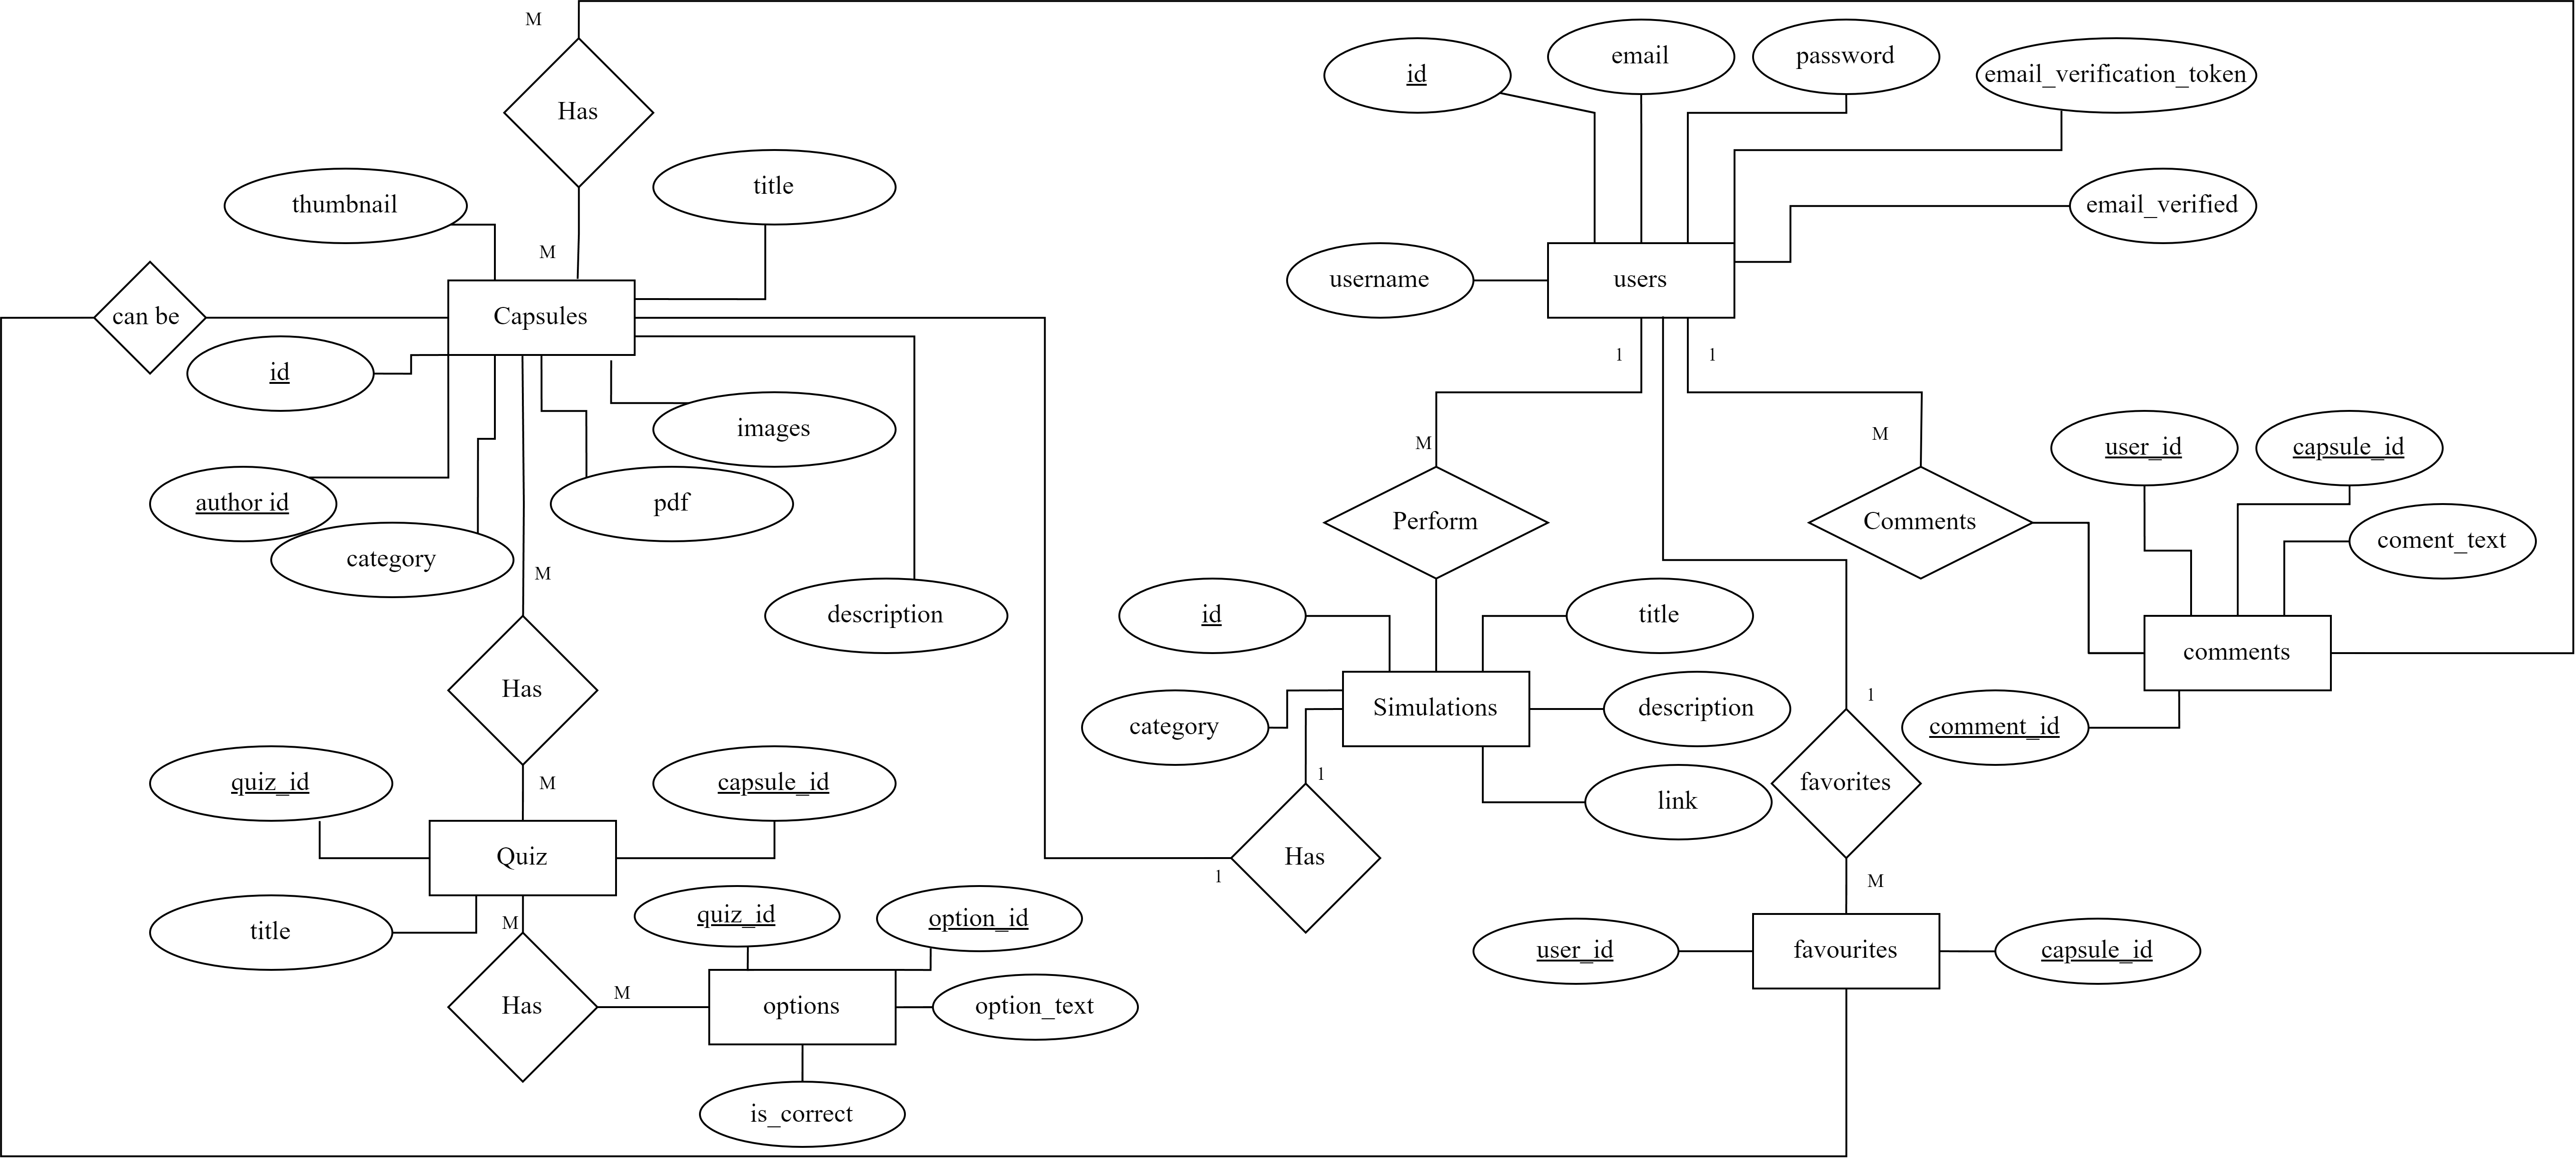
\includegraphics[height = 14cm]{Diagrams/er.drawio.png}}
    \caption{ER Diagram of System Data}
\end{figure}
\newpage
\section{Structured System Design}
\subsection{Architecture Design}
The following diagram shows diagram of our Architecture. Mainly shows what are the functions can be accessed after starting our application.
\begin{figure}[H]
    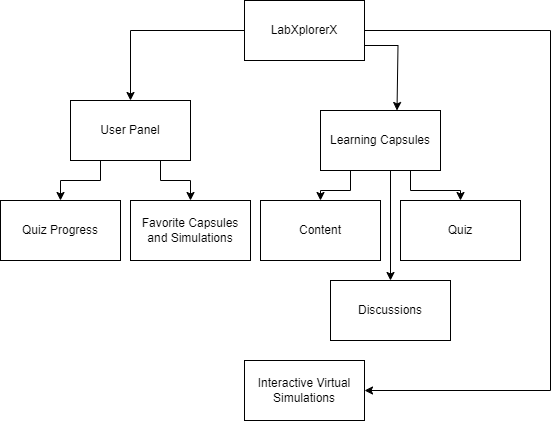
\includegraphics[height = 5.7cm]{Diagrams/Main_Block.png}
    \caption{Main Architecture of System}
\end{figure}
\newpage
\subsection{Database Schema Design}
An activity diagram visually presents a series of actions or flow of control in a system similar to a flowchart or a data flow diagram. This diagram showed how our program flow goes on.
\begin{figure}[H]
   \centering
    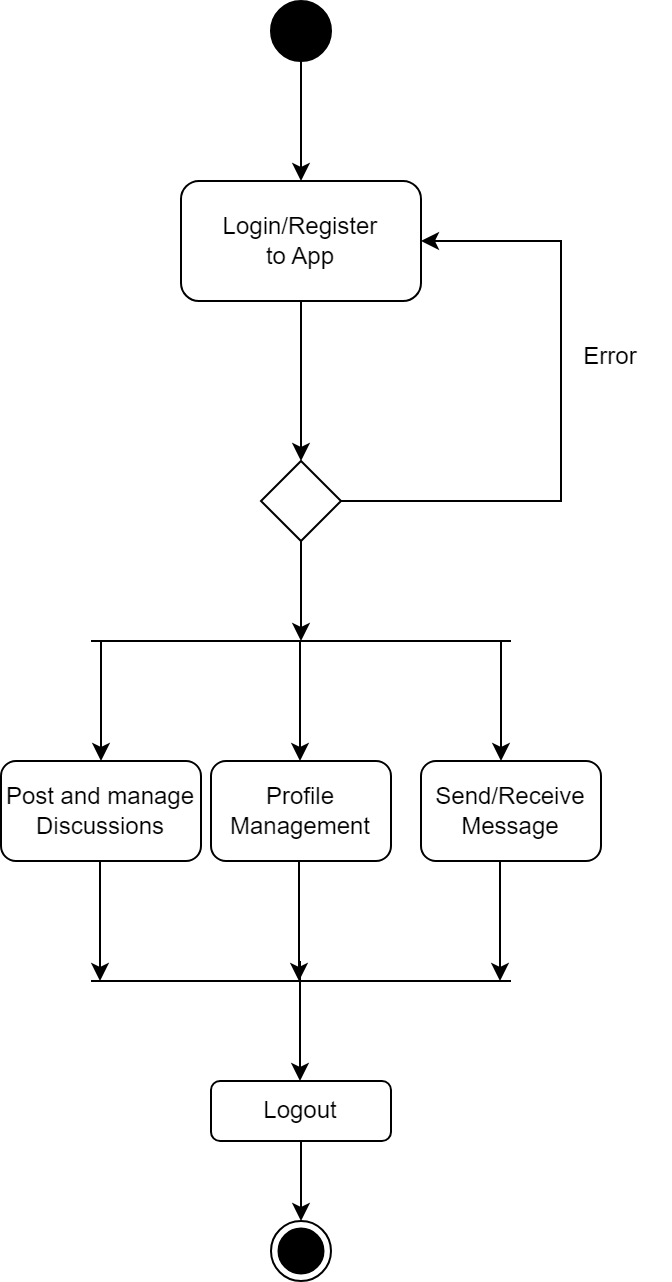
\includegraphics[height = 15cm]{Diagrams/Activity.drawio.png}
    \caption{Activity Diagram}
\end{figure}
\newpage

\subsection{Interface Design}
An activity diagram visually presents a series of actions or flow of control in a system similar to a flowchart or a data flow diagram. This diagram showed how our program flow goes on.
\begin{figure}[H]
   \centering
    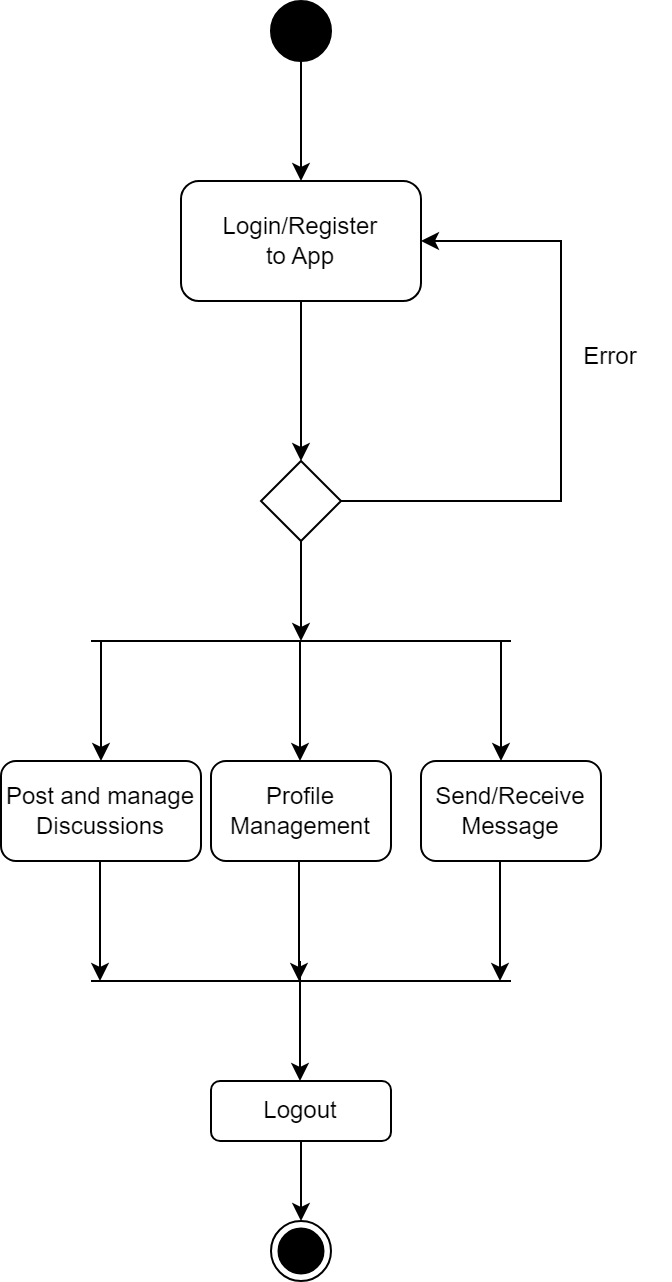
\includegraphics[height = 15cm]{Diagrams/Activity.drawio.png}
    \caption{Activity Diagram}
\end{figure}
\newpage
\subsection{Physical DFD}
DFD or Data Flow Diagram is mainly used to show how data are being flowed in and out of our system. There are 3 levels of DFD i.e Context Level(Level 0),Level 1 and Level 2
\begin{figure}[H]
    \centering
    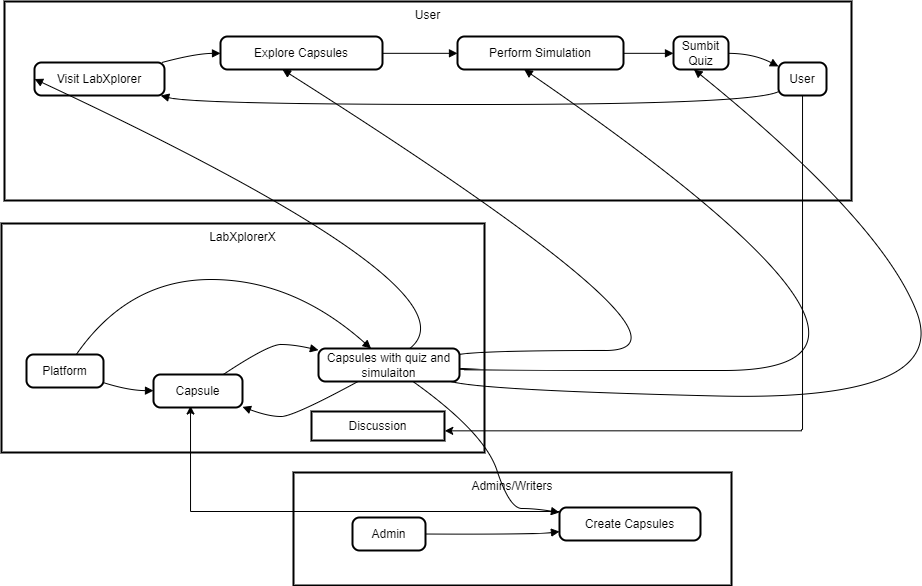
\includegraphics[height = 9cm]{Diagrams/DFD.drawio.png}
    \caption{Data Flow Diagram (Context Level)}
\end{figure}
\newpage
\section{Algorithm Details}